\documentclass{article}
\usepackage{tikz}
\usetikzlibrary{matrix}

\begin{document}

\begin{figure}[h]
    \centering
    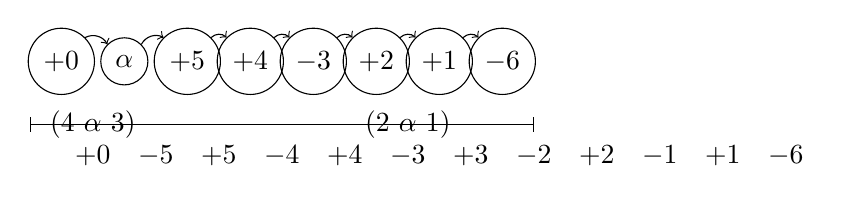
\begin{tikzpicture}[scale=0.8]
        % Define the nodes
        \node[circle,draw] (0) at (0,0) {$+0$};
        \node[circle,draw] (a) at (1,0) {$\alpha$};
        \node[circle,draw] (5) at (2,0) {$+5$};
        \node[circle,draw] (4) at (3,0) {$+4$};
        \node[circle,draw] (3) at (4,0) {$-3$};
        \node[circle,draw] (2) at (5,0) {$+2$};
        \node[circle,draw] (1) at (6,0) {$+1$};
        \node[circle,draw] (6) at (7,0) {$-6$};

        % Draw the edges
        \draw[->] (0) to[bend left=45] (a);
        \draw[->] (a) to[bend left=45] (5);
        \draw[->] (5) to[bend left=45] (4);
        \draw[->] (4) to[bend left=45] (3);
        \draw[->] (3) to[bend left=45] (2);
        \draw[->] (2) to[bend left=45] (1);
        \draw[->] (1) to[bend left=45] (6);

        % Draw the horizontal line
        \draw[|-|] (-0.5,-1) -- (7.5,-1);
        \node at (0.5,-1) {$(4~\alpha~3)$};
        \node at (5.5,-1) {$(2~\alpha~1)$};

        % Draw the labels
        \node at (0.5,-1.5) {$+0$};
        \node at (1.5,-1.5) {$-5$};
        \node at (2.5,-1.5) {$+5$};
        \node at (3.5,-1.5) {$-4$};
        \node at (4.5,-1.5) {$+4$};
        \node at (5.5,-1.5) {$-3$};
        \node at (6.5,-1.5) {$+3$};
        \node at (7.5,-1.5) {$-2$};
        \node at (8.5,-1.5) {$+2$};
        \node at (9.5,-1.5) {$-1$};
        \node at (10.5,-1.5) {$+1$};
        \node at (11.5,-1.5) {$-6$};
    \end{tikzpicture}

    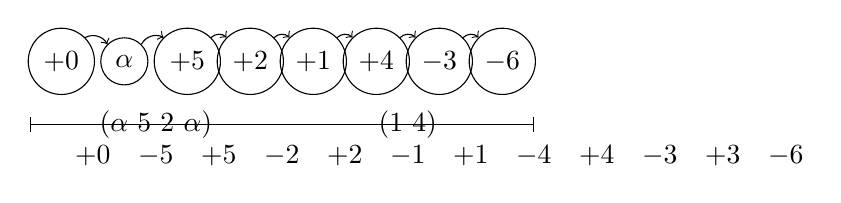
\begin{tikzpicture}[scale=0.8]
        % Define the nodes
        \node[circle,draw] (0) at (0,0) {$+0$};
        \node[circle,draw] (a) at (1,0) {$\alpha$};
        \node[circle,draw] (5) at (2,0) {$+5$};
        \node[circle,draw] (2) at (3,0) {$+2$};
        \node[circle,draw] (1) at (4,0) {$+1$};
        \node[circle,draw] (4) at (5,0) {$+4$};
        \node[circle,draw] (3) at (6,0) {$-3$};
        \node[circle,draw] (6) at (7,0) {$-6$};

        % Draw the edges
        \draw[->] (0) to[bend left=45] (a);
        \draw[->] (a) to[bend left=45] (5);
        \draw[->] (5) to[bend left=45] (2);
        \draw[->] (2) to[bend left=45] (1);
        \draw[->] (1) to[bend left=45] (4);
        \draw[->] (4) to[bend left=45] (3);
        \draw[->] (3) to[bend left=45] (6);

        % Draw the horizontal line
        \draw[|-|] (-0.5,-1) -- (7.5,-1);
        \node at (1.5,-1) {$(\alpha~5~2~\alpha)$};
        \node at (5.5,-1) {$(1~4)$};

        % Draw the labels
        \node at (0.5,-1.5) {$+0$};
        \node at (1.5,-1.5) {$-5$};
        \node at (2.5,-1.5) {$+5$};
        \node at (3.5,-1.5) {$-2$};
        \node at (4.5,-1.5) {$+2$};
        \node at (5.5,-1.5) {$-1$};
        \node at (6.5,-1.5) {$+1$};
        \node at (7.5,-1.5) {$-4$};
        \node at (8.5,-1.5) {$+4$};
        \node at (9.5,-1.5) {$-3$};
        \node at (10.5,-1.5) {$+3$};
        \node at (11.5,-1.5) {$-6$};
    \end{tikzpicture}

    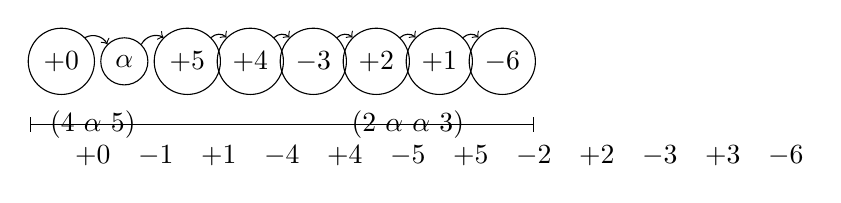
\begin{tikzpicture}[scale=0.8]
        % Define the nodes
        \node[circle,draw] (0) at (0,0) {$+0$};
        \node[circle,draw] (a) at (1,0) {$\alpha$};
        \node[circle,draw] (5) at (2,0) {$+5$};
        \node[circle,draw] (4) at (3,0) {$+4$};
        \node[circle,draw] (3) at (4,0) {$-3$};
        \node[circle,draw] (2) at (5,0) {$+2$};
        \node[circle,draw] (1) at (6,0) {$+1$};
        \node[circle,draw] (6) at (7,0) {$-6$};

        % Draw the edges
        \draw[->] (0) to[bend left=45] (a);
        \draw[->] (a) to[bend left=45] (5);
        \draw[->] (5) to[bend left=45] (4);
        \draw[->] (4) to[bend left=45] (3);
        \draw[->] (3) to[bend left=45] (2);
        \draw[->] (2) to[bend left=45] (1);
        \draw[->] (1) to[bend left=45] (6);

        % Draw the horizontal line
        \draw[|-|] (-0.5,-1) -- (7.5,-1);
        \node at (0.5,-1) {$(4~\alpha~5)$};
        \node at (5.5,-1) {$(2~\alpha~\alpha~3)$};

        % Draw the labels
        \node at (0.5,-1.5) {$+0$};
        \node at (1.5,-1.5) {$-1$};
        \node at (2.5,-1.5) {$+1$};
        \node at (3.5,-1.5) {$-4$};
        \node at (4.5,-1.5) {$+4$};
        \node at (5.5,-1.5) {$-5$};
        \node at (6.5,-1.5) {$+5$};
        \node at (7.5,-1.5) {$-2$};
        \node at (8.5,-1.5) {$+2$};
        \node at (9.5,-1.5) {$-3$};
        \node at (10.5,-1.5) {$+3$};
        \node at (11.5,-1.5) {$-6$};
    \end{tikzpicture}

    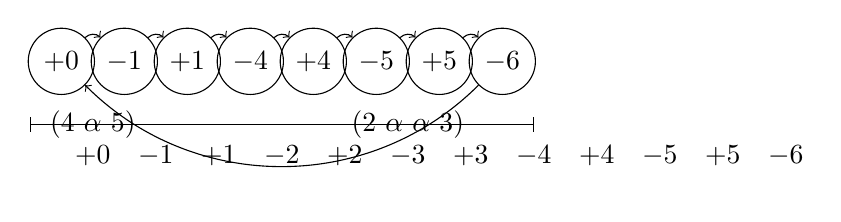
\begin{tikzpicture}[scale=0.8]
        % Define the nodes
        \node[circle,draw] (0) at (0,0) {$+0$};
        \node[circle,draw] (1) at (1,0) {$-1$};
        \node[circle,draw] (2) at (2,0) {$+1$};
        \node[circle,draw] (3) at (3,0) {$-4$};
        \node[circle,draw] (4) at (4,0) {$+4$};
        \node[circle,draw] (5) at (5,0) {$-5$};
        \node[circle,draw] (6) at (6,0) {$+5$};
        \node[circle,draw] (7) at (7,0) {$-6$};

        % Draw the edges
        \draw[->] (0) to[bend left=45] (1);
        \draw[->] (1) to[bend left=45] (2);
        \draw[->] (2) to[bend left=45] (3);
        \draw[->] (3) to[bend left=45] (4);
        \draw[->] (4) to[bend left=45] (5);
        \draw[->] (5) to[bend left=45] (6);
        \draw[->] (6) to[bend left=45] (7);
        \draw[->] (7) to[bend left=45] (0);

        % Draw the horizontal line
        \draw[|-|] (-0.5,-1) -- (7.5,-1);
        \node at (0.5,-1) {$(4~\alpha~5)$};
        \node at (5.5,-1) {$(2~\alpha~\alpha~3)$};

        % Draw the labels
        \node at (0.5,-1.5) {$+0$};
        \node at (1.5,-1.5) {$-1$};
        \node at (2.5,-1.5) {$+1$};
        \node at (3.5,-1.5) {$-2$};
        \node at (4.5,-1.5) {$+2$};
        \node at (5.5,-1.5) {$-3$};
        \node at (6.5,-1.5) {$+3$};
        \node at (7.5,-1.5) {$-4$};
        \node at (8.5,-1.5) {$+4$};
        \node at (9.5,-1.5) {$-5$};
        \node at (10.5,-1.5) {$+5$};
        \node at (11.5,-1.5) {$-6$};
    \end{tikzpicture}
\end{figure}

\caption{Exemplo de uma sequência de transposições que agem em dois ciclos não orientados \( C = (5, 3, 1) \) e \( D = (6, 4, 2) \), tal que \( C \) é rotulado e \( D \) é limpo. Essas operações criam três novos ciclos limpos. Neste exemplo, temos \( A = (0~\alpha~5~4~\alpha~3~2~\alpha~1~6) \) e \( \iota^n \) com \( n = 5 \).}

\end{document}